\documentclass[12pt, a4paper]{article}
\usepackage{ctex}
\usepackage{amsmath}
\usepackage{amsfonts}
\usepackage{amsthm}
\usepackage{graphicx}
\usepackage{theorem}
\usepackage{hyperref}
\usepackage[a4paper, left=2cm, top=2cm, total={170mm, 257mm}]{geometry}
\usepackage{verbatim}
\usepackage{listings}
\usepackage{fontspec}
\usepackage{color}
\usepackage{caption}
\usepackage{float}
\setsansfont{Consolas}
\setmonofont{Fira Code}
\setCJKmainfont{Sarasa UI SC}
\setCJKsansfont{Sarasa Term SC}
\setCJKmonofont{Sarasa Mono SC}
\title{吴恩达机器学习读书笔记 \\ Machine Learning by Andrew Ng}
\author{Zhaorui.Zhan}
\date{}
\begin{document}
    \maketitle

    \begin{abstract}    
        基于吴恩达在Coursera上的公开课Machine Learning做的笔记。对定性部分进行了一些省略,重点关注算法的使用与逻辑推导。
    \end{abstract}

    \tableofcontents
    \newpage

    \section{引言 Introduction}

        监督学习是给学习算法的一个数据集中,数据集样本本身已经提供了“正确答案”,需要根据这些样本做出预测。而无监督学习中,数据集没有任何标签,需要算法根据数据集本身对其进行分类或标记,从而找出某种结构。

        针对连续值的预测称为回归问题,对于离散值的预测称为分类问题。

    \section{单变量线性回归 Linear Regression with One Variable}

        \subsection{模型表示}
            对于回归问题的标记,通常定义为:

            \begin{enumerate}
                \item $m$:训练集中实例的数量(有多少个样本)
                \item $y$:特征/输入变量
                \item $(x, y)$:目标变量/输出变量
                \item $(x^{(i)}, y^{(i)})$:第$i$个观测实例
                \item $h$:学习算法的函数,也称为假设\textit{hypothesis}
            \end{enumerate}

            最简单的预测方式为$h_\theta(x)=\theta_0 + \theta_1x$,因为只含有一个特征变量,因此这种问题被称为单变量线性回归问题。

        \subsection{代价函数}
            当已经创建了假设函数,即用来预测的函数形式为:$h_\theta(x)=\theta_0 + \theta_1x$,后续的问题是如何对使用的模型选择合适的参数$\theta_i$。在单变量线性回归中,需要选择的就是直线的斜率$\theta_1$和截距项$\theta_0$。

            由于选择的参数决定了得到的模型对应的直线相对于训练集的准确程度,模型所预测的值与训练集中实际值的差异就是建模误差\textit{modelling error},即$y_i - \hat{y}_i$。

            选择参数的过程就是选择将建模误差的平方和最小的参数。
            
            在这里定义代价函数$J(\theta_0, \theta_1)$,当$J(\theta_0, \theta_1)$最小时,选择的参数为最优参数。即:

            \begin{align*}
                &\mathbf{Hypothesis}: h_\theta(x)=\theta_0 + \theta_1x \\
                &\mathbf{Cost Function}: J(\theta_0, \theta_i) = \frac{1}{2m}\sum_{i=1}^{m}(h_\theta(x^{(i)})-y^{(i)})^2 \\
                &\mathbf{Goal}: \mathop{minimize}\limits_{\theta_0, \theta_1}J(\theta_0, \theta_1)
            \end{align*}

            对上述代价函数进行简化,假设$\theta_0=0$,同时只有三个样本点$(1,1),(2,2),(3,3)$:

            对于这个简化的模型,可以选择无数个$\theta_1$进行模拟:
            
            \begin{enumerate}
                \item $\theta_1=0$
                \begin{align*}
                    &h_\theta(x) = 0 \\
                    &J(0) = \frac{1}{2*3}(-1^2+-2^2+-3^2) = \frac{14}{6}
                \end{align*}
                \item $\theta_1=0.5$
                \begin{align*}
                    &h_\theta(x) = 0.5x \\
                    &J(0) = \frac{1}{2*3}(-0.5^2+-1^2+-1.5^2) = \frac{3.5}{6}
                \end{align*}
                \item $\theta_1=1$
                \begin{align*}
                    &h_\theta(x) = x \\
                    &J(0) = \frac{1}{2*3}(0^2+0^2+0^2) = 0
                \end{align*}
                \item $\dots$
            \end{enumerate}

            \begin{figure}[H]
                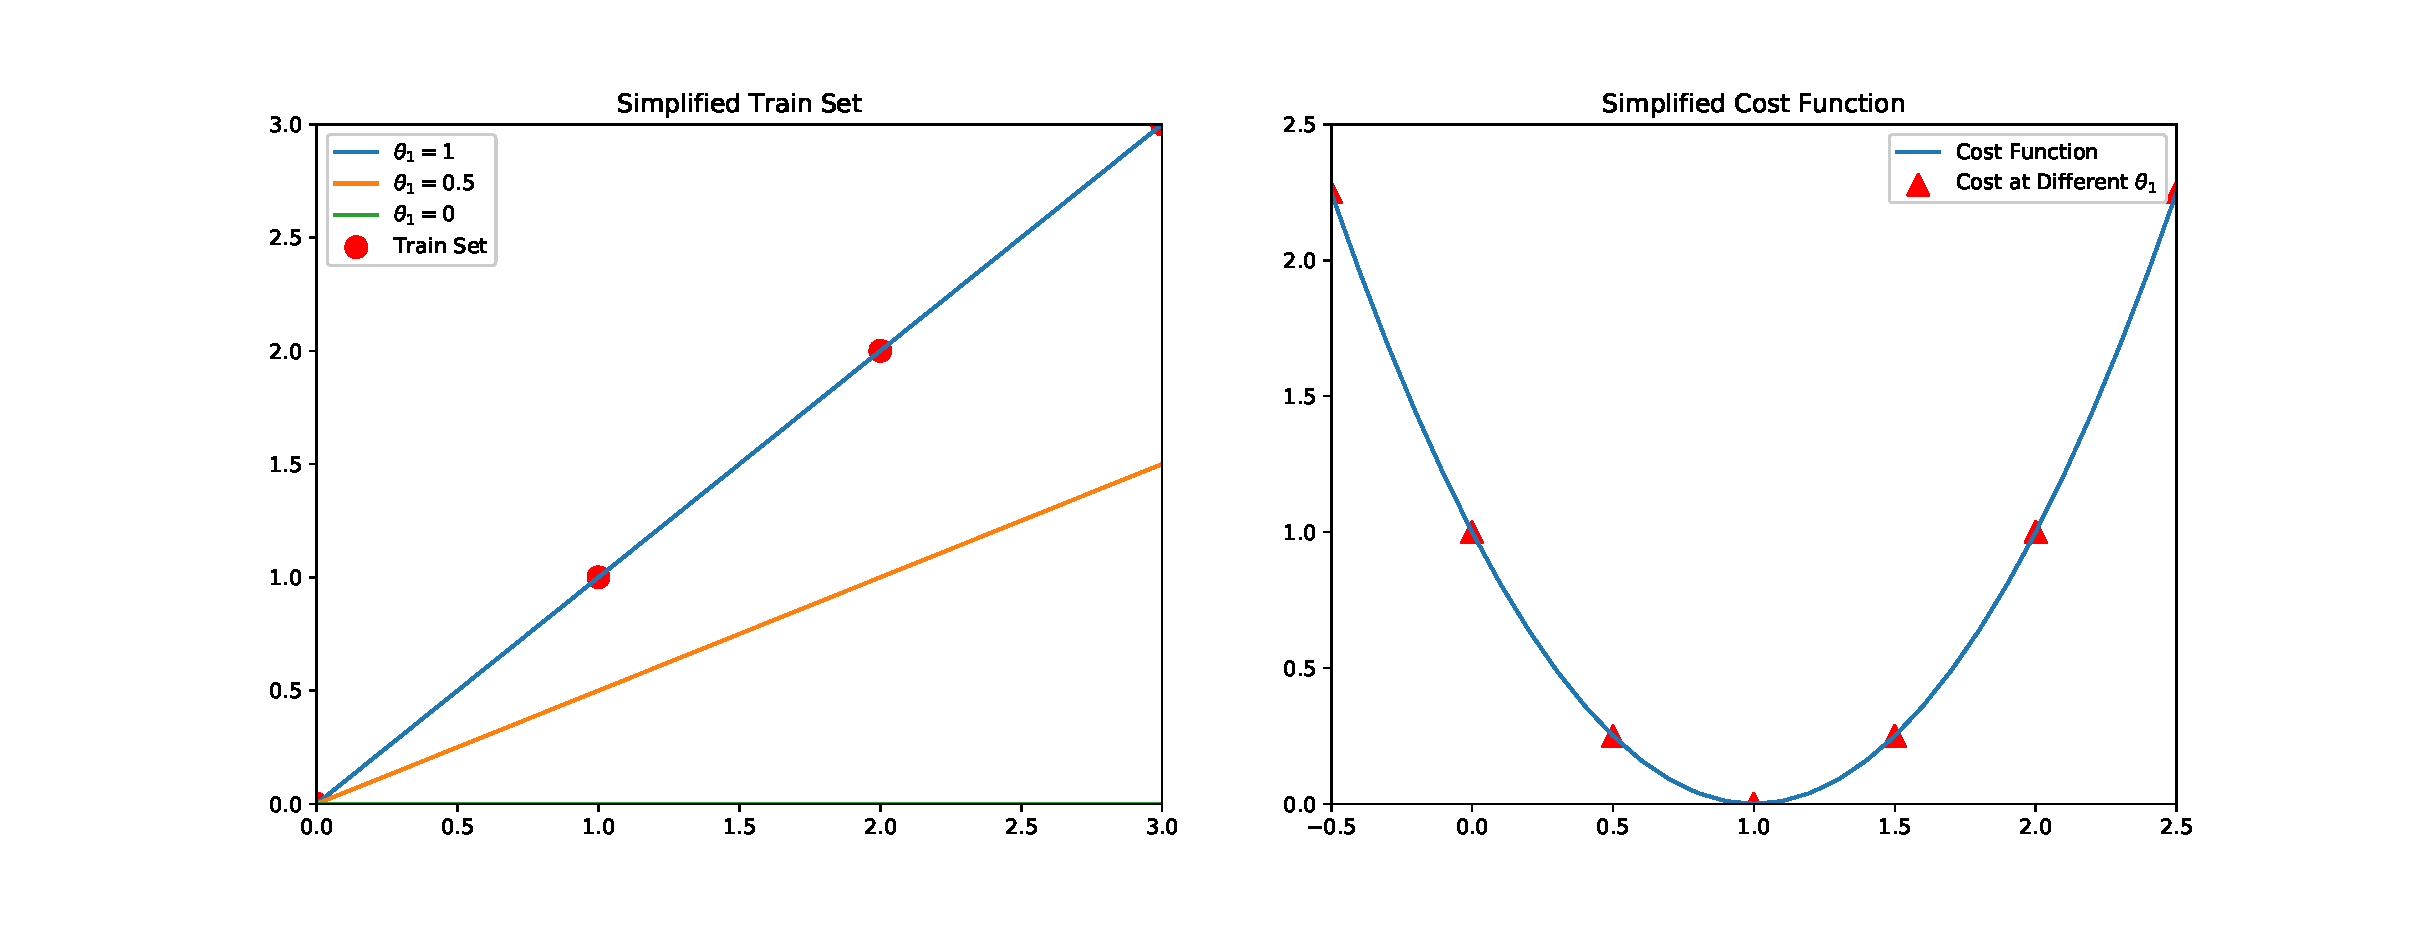
\includegraphics[width=1\textwidth]{OneParameterCostFunction.eps}
            \end{figure}

            将这些点连在一起形成的曲线,就构成了一个参数下的代价函数曲线。实际上,将三个样本点带入后,可以得到这里的代价函数$J(\theta_1)$的解析式为$J(\theta_1)=\frac{14}{6}(\theta_1-1)^2$。

            


    \section{线性代数回顾 Linear Algebra Review}

    \section{多变量线性回归 Linear Regression with Multiple Variables}

    \section{Octave教程 Octave Tutorial}

    \section{逻辑回归 Logistic Regression}

    \section{正则化 Regularization}

    \section{神经网络:表述 Neural Networks: Representation}

    \section{神经网络:学习 Neural Networks: Learning}
    
    \section{应用机器学习的建议 Advice for Apply Machine Learning}

    \section{机器学习系统的设计 Machine Learning System Design}

    \section{支持向量机 Support Vector Machines}

    \section{聚类 Clustering}

    \section{降维 Dimensionality Reduction}

    \section{异常检测 Anomaly Detection}

    \section{推荐系统 Recommender Systems}

    \section{大规模机器学习 Large Scale Machine Learning}

    \section{结语 Conclusion}

\end{document}